% !TeX spellcheck = en_US
\newpage
\section{Clustering}
Clusters may carry important insights about the system or the process that generates the data such as the existence of different \textbf{states} (healthy or sick) or different \textbf{subprocesses}.

\begin{example}
	Methylation profiles of cancer cells organized into clusters, which often correlates with oncology categories. 
	
	\begin{center}
		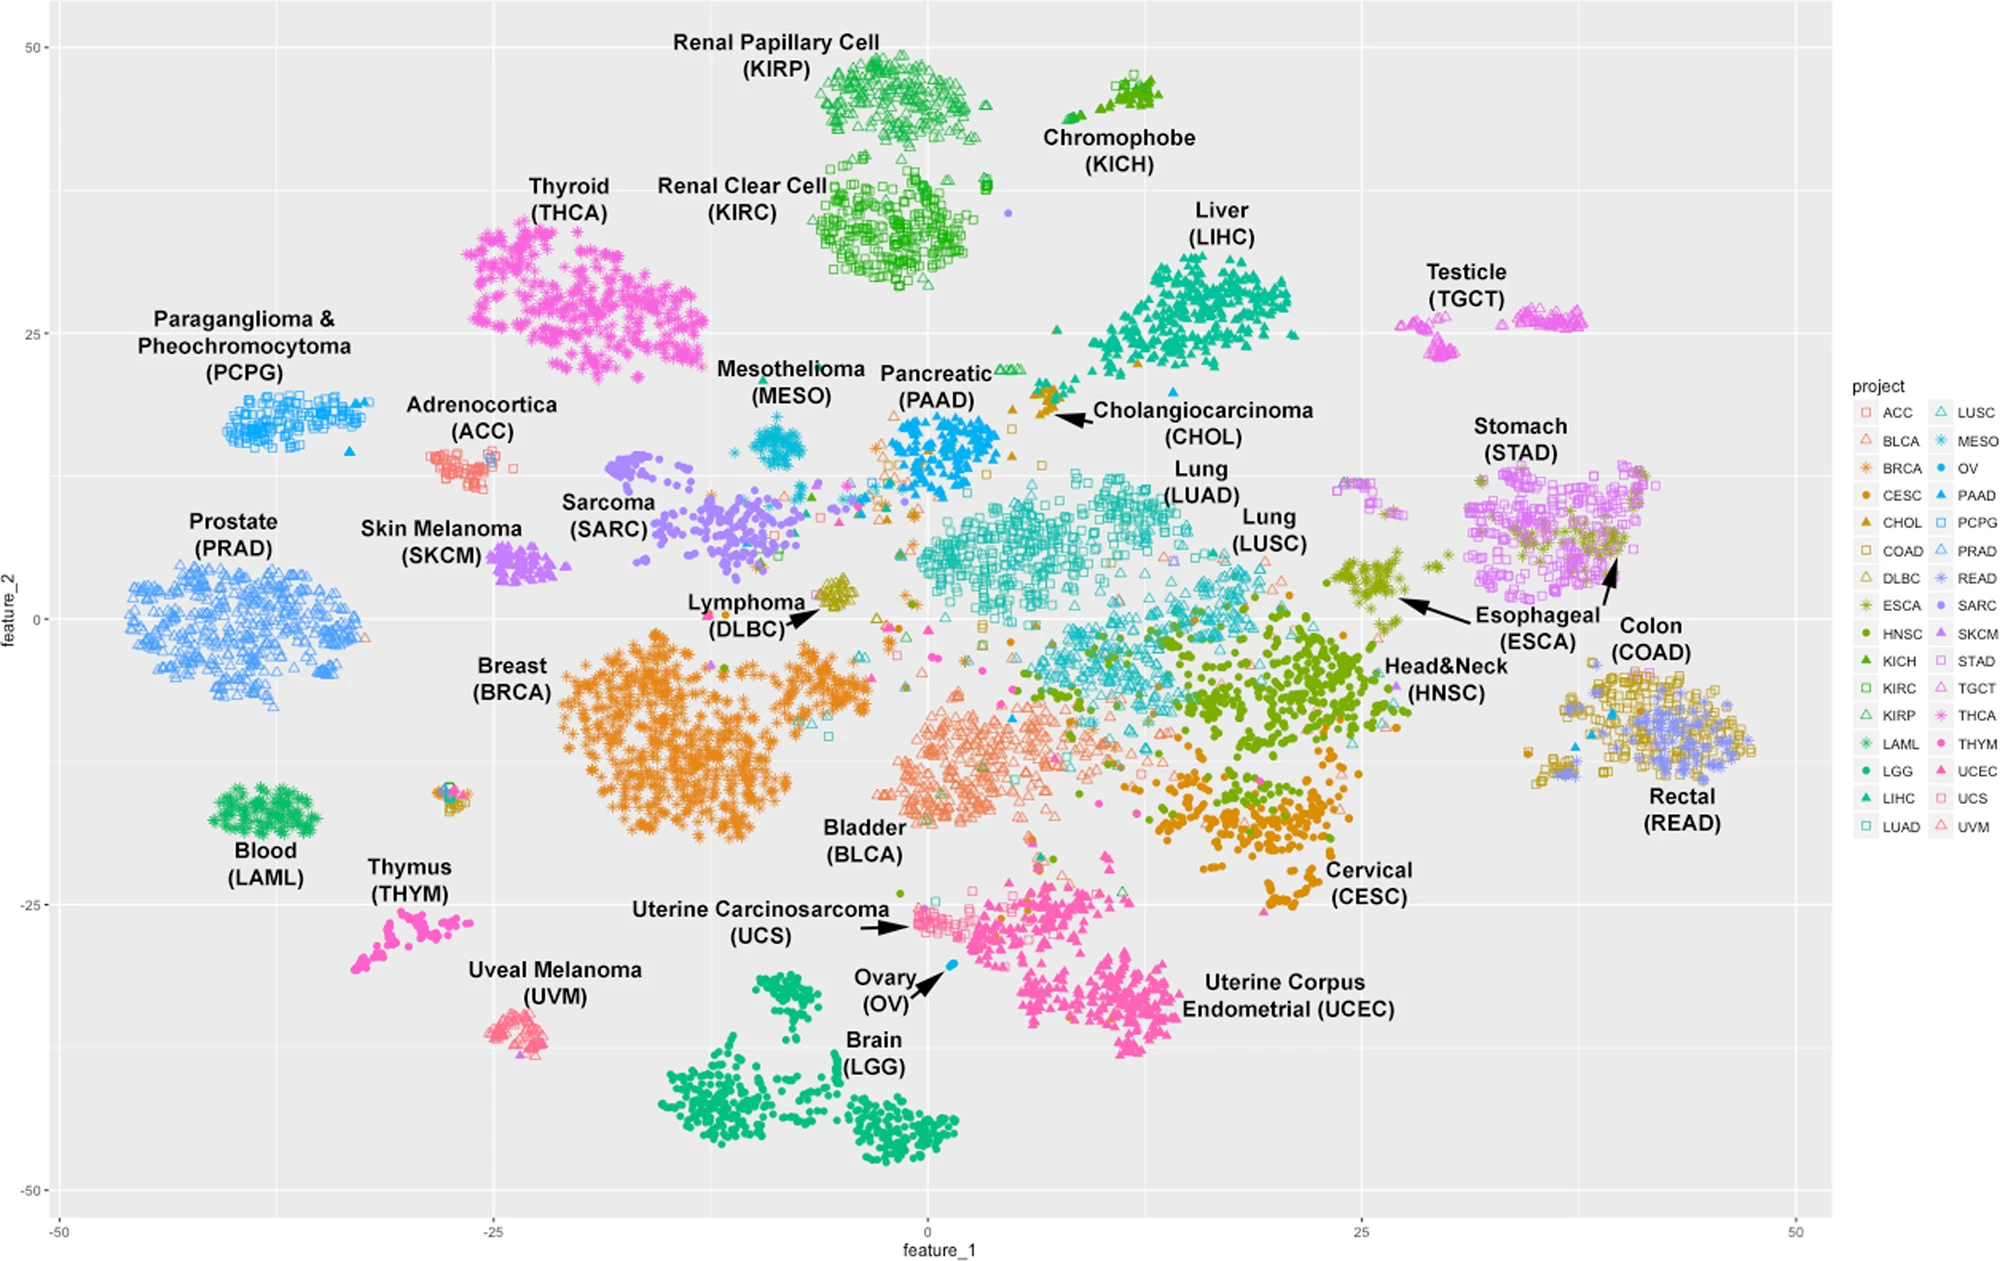
\includegraphics[scale=0.2]{clusters}
	\end{center}
\end{example}

\subsection{K-Means}
In the \textbf{centroid model} each cluster $k$ is represented by a \textbf{centroid} $\mu_k$ that lies in the same $d$-dimensional space as the data. It represents a prototype for points in that cluster, which are typically close to it.\\
The most well-known centroid-based technique is the \textbf{K-Means} algorithm, which works by iteratively updating the centroids and the assigned points until convergence.
\subsubsection{Algorithm}
Assuming a dataset $x_1, \ldots, x_N$, let $c_i \in \{1, \ldots, K\}$ be the cluster to which instance $i$ is assigned and let $C_k = \{i: c_i = k\}$ denote the set of instances in cluster $k$. Each cluster is represented by a centroid $\mu_k$ initialized at random. The algorithm is:
\begin{lstlisting}[mathescape=true]
	repeat
		$\forall_{i=1}^N: c_i = \arg\min_k \lvert\lvert \mathbf{x}_i - \mathbf{\mu}_k\rvert\rvert^2$
		$\forall_{i=1}^N: c_i = \mathbf{\mu}_k \leftarrow \frac{1}{\lvert C_k \rvert} \sum_{i \in C_k} \mathbf{x}_i$
	until convergence
\end{lstlisting}
\subsubsection{Optimization problem}
The algorithm can be interpreted as an attempt to \textbf{minimize}
\begin{equation}
	J(\mathbf{\mu}, \mathbf{c}) = \sum_{i=1}^N\lvert\lvert \mathbf{x}_i - \mathbf{\mu}_{c_i}\rvert\rvert^2 = \sum_{k=1}^K\sum_{i\in C_k}\lvert\lvert \mathbf{x}_i - \mathbf{\mu}_{k}\rvert\rvert^2
\end{equation}
which quantifies the amount of \textbf{dispersion} in each cluster.
\newpage
\noindent The \textbf{proof} for the two steps are:
\begin{enumerate}
	\item The objective is \textbf{sum-decomposable} with $c_1, c_2, \ldots, c_N$ and each cluster assignment can be optimized independently
	\begin{equation*}
		\arg\min_\mathbf{c} \sum_{i=1}^N \lvert\lvert \mathbf{x}_i - \mathbf{\mu}_{c_i}\rvert\rvert^2 = (\arg\min_{c_i}\lvert\lvert \mathbf{x}_i - \mathbf{\mu}_{c_i}\rvert\rvert^2)^N_{i=1}
	\end{equation*}
	\item Objective is also \textbf{sum-decomposable} with cluster prototypes and each of them can be optimized independently
	\begin{equation*}
		\arg\min_\mathbf{\mu}\sum_{k=1}^K\sum_{i\in C_k}\lvert\lvert \mathbf{x}_i - \mathbf{\mu}_{k}\rvert\rvert^2 = (\arg\min_{\mathbf{\mu}_k}\sum_{i\in C_k}\lvert\lvert \mathbf{x}_i - \mathbf{\mu}_{k}\rvert\rvert^2)^K_{k=1}
	\end{equation*}
\end{enumerate}

\begin{note}
	The clustering produced by the K-Means algorithm can be modeled by a \textbf{Voronoi diagram}.
	\begin{center}
		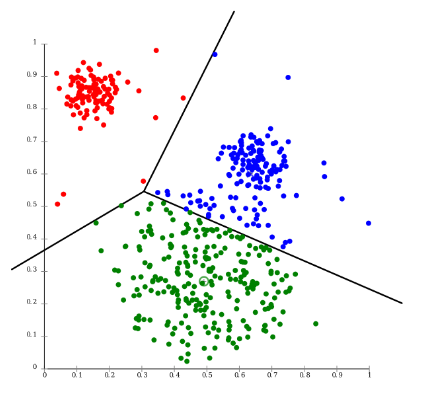
\includegraphics[scale=0.2]{voronoi}
	\end{center}
\end{note}

\subsubsection{Explained variance}
Data dispersion can be decomposed as follows:
\begin{align*}
	\frac{1}{N} \sum_{i=1}^{N} \lvert\lvert \mathbf{x}_i - \mathbf{\mu} \rvert\rvert^2 & = \frac{1}{N} \sum_k \sum_{i\in C_k} \lvert\lvert \mathbf{x}_i - \mathbf{\mu} \rvert\rvert^2\\
	& = \frac{1}{N} \sum_k \sum_{i\in C_k} \lvert\lvert \mathbf{x}_i - \mathbf{\mu}_k + \mathbf{\mu}_k - \mathbf{\mu} \rvert\rvert^2 \\
	& = \frac{1}{N} \sum_k \sum_{i\in C_k} [\lvert\lvert \mathbf{x}_i - \mathbf{\mu}_k\rvert\rvert^2 + \lvert\lvert \mathbf{\mu}_k - \mathbf{\mu} \rvert\rvert^2 +2(\mathbf{x}_i -\mathbf{\mu}_k)^T(\mathbf{\mu}_k - \mathbf{\mu})]\\
	& = \underbrace{\frac{1}{N} \sum_k \sum_{i\in C_k} \lvert\lvert \mathbf{x}_i - \mathbf{\mu}_k\rvert\rvert^2}_{\text{within-cluster dispersion}} + \underbrace{\frac{1}{N} \sum_k \sum_{i\in C_k} \lvert\lvert \mathbf{\mu}_k - \mathbf{\mu} \rvert\rvert^2}_{\text{between-cluster dispersion}} + \underbrace{\frac{2}{N} \sum_k \sum_{i\in C_k} +(\mathbf{x}_i -\mathbf{\mu}_k)^T(\mathbf{\mu}_k - \mathbf{\mu})}_{0}
\end{align*}
We define the \textbf{Calinski-Harabasz Index} as a criterion for evaluating the quality of a clustering solution. It's represented by the ratio of \textit{within-cluster dispersion} over \textit{between-cluster dispersion} multiplied by model simplicity:
\begin{equation}
	\text{Calinski-Harabasz}=\underbrace{\frac{\sum_k \sum_{i\in C_k} \lvert\lvert \mathbf{x}_i - \mathbf{\mu}_k\rvert\rvert^2}{\sum_k \sum_{i\in C_k} \lvert\lvert \mathbf{\mu}_k - \mathbf{\mu} \rvert\rvert^2}}_{\text{Model descriptive power}}\cdot \underbrace{\frac{N- K}{K-1}}_{\text{Model simplicity}}
\end{equation}
\paragraph{Choosing K} For a constant number of $K$ clusters, the algorithm optimizes the Calinski-Harabasz index. At the same time it helps on how to set that parameter. There are two approaches:
\begin{itemize}
	\item \textbf{Maximizing the index}: consider that the \textit{within-cluster dispersion} favors large $K$ while \textit{model simplicity} penalizes large $K$
	\item Looking for an \textbf{inflection} in the explained variance
	\begin{equation}
		\text{ExpVar}(\%) = \frac{\frac{1}{N} \sum_k \sum_{i\in C_k} \lvert\lvert \mathbf{\mu}_k - \mathbf{\mu} \rvert\rvert^2}{{\frac{1}{N}\sum_{i=1}^N \lvert\lvert \mathbf{x} - \mathbf{\mu}\rvert\rvert^2}}
	\end{equation}
\end{itemize}

\subsubsection{Limits}
K-Means has the following limits:
\begin{itemize}
	\item \textbf{Non convexity}: you initialize with values of the centroids that cover well the data. You repeat from $1$ to $100$ times and keep the solution that reaches the lowest objective
	\item \textbf{Low descriptive power}: even if the selected number of clusters is correct and the true optimum is reached, the solution may not be a desirable one, because the algorithm focuses on finding the clusters with least dispersion without paying attention to other aspects such as the margins between clusters
\end{itemize}

\subsection{Spectral clustering}
The dataset $\mathcal{D}$ is first converted into a \textbf{graph} $\mathcal{G}$ with an \textbf{adjacency matrix} $A$ indicating whether the distance between pair of points is below a certain threshold.\\
Then we need to find the \textbf{connected components} in the graph through an analysis of the adjacency matrix. To do that we:
\begin{enumerate}
	\item Represent $\mathcal{G}$ by the adjacency matrix $A$
	\item Build a derived matrix called \textbf{Laplacian}
	\begin{equation*}
		L = D-A
	\end{equation*}
	where $D=\text{diag}(A \cdot \mathbf{1})$ is the \textbf{degree matrix} and $\mathbf{1}$ is a vector of ones
	\item Perform \textbf{eigenvalue decomposition} of $L$, that is solving $L\mathbf{u} = \lambda \mathbf{u}$
	\item Eigenvectors $\mathbf{u}$ associated to eigenvalues $\lambda = 0$ are indicator vectors for the various connected components 
\end{enumerate}
\subsubsection{Formal derivation}
We can interpret the eigenvalues as the \textbf{variation of the eigenvector elements} between connected nodes. If $\lambda=0$, the eigenvector elements should be constant for each connected component.
\begin{align*}
	\lambda & = \mathbf{u}^TL\mathbf{u}\\
	& = \mathbf{u}^T(D-A)\mathbf{u}\\
	& = \sum_{i=1}^{N} \sum_{j=1}^{N} u_id_{ij}u_j - u_ia_{ij}u_j\\
	& = \qquad \vdots \\
	& = \frac{1}{2} \sum_{i=1}^{N} \sum_{j=1}^{N} a_{ij} (u_i - u_j)^2
\end{align*}

\begin{theorem}
	The number of zero eigenvalues of the Laplacian $L$, that is the multiplicity of the $0$ eigenvalue, equals the number of connected components $K$ of the graph.
\end{theorem}

The \textbf{last equation}, this \textbf{theorem} and the fact that \textbf{eigenvectors are orthogonal}, imply that the set of eigenvector with zero eigenvalue are indicator vectors for the connected components. Therefore, cluster membership is obtained by finding points that are embedded in the exact same location in eigenvector space.

\begin{center}
	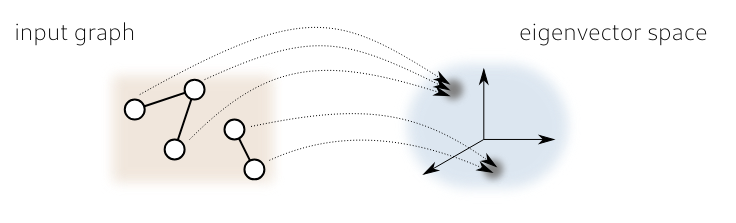
\includegraphics[scale=0.3]{clustin}
\end{center}

\subsubsection{Cheeger's Inequality}
\paragraph{Conductance}
Given the \textbf{conductance} of some set vertices $\mathcal{S}$ in the graph $\mathcal{G}$
\begin{equation}
	\phi(\mathcal{S}) = \frac{\text{edges}(\mathcal{S}, \overline{\mathcal{S}})}{\sum_{v \in \mathcal{S}}\text{degree}(v)}
\end{equation}
the conductance of the whole graph is defined as the minimum one among the sets that have at most half the volume of the complete graph
\begin{equation}
	\phi(\mathcal{G}) = \min_{\mathcal{S}:\text{vol}(\mathcal{S}) \leq \frac{\text{vol}(\mathcal{V})}{2}}\phi(\mathcal{S})
\end{equation}

\begin{definition}[Cheeger's Inequality]
	Let $\phi(\mathcal{G})$ denote the conductance of the graph $\mathcal{G}$. Then that can be related to the Laplacian's second eigenvalue as
	\begin{equation}
		\frac{\lambda2}{2} \leq \phi(\mathcal{G}) \leq \sqrt{2 \lambda_2}
	\end{equation}
\end{definition}

This inequality \textbf{implies} that if the conductance is low (natural 2-clustering), then the second eigenvalue $\lambda_2$ is low. Furthermore we can deduce that a low $\lambda_2$ will correspond to to low variations of the corresponding eigenvectors along connected nodes, hence it's predictive of cluster membership.

\subsubsection{Practice}
In practice spectral clustering can capture general cluster structures, including the ones that are non linearly separable. The quality of the clusters can substantially decrease if the data is noisy, but this is addressable through:
\begin{itemize}
	\item \textbf{Adjacency matrix}: try different parameters and ways of building it
	\begin{itemize}
		\item \textbf{Distance cutout}
		\begin{equation*}
			a_{ij}=I(\lvert\lvert \mathbf{x}_i - \mathbf{x}_j\rvert\rvert < \delta)
		\end{equation*}
		\item \textbf{Nearest neighbor}
		\item \textbf{Radial basis function}
		\begin{equation*}
			a_{ij} = \exp(- \frac{\lvert\lvert \mathbf{x}_i -\mathbf{x}_j \rvert\rvert}{2 \sigma^2} )
		\end{equation*}
	\end{itemize}
	\item \textbf{Laplacian matrix}: a variant of the standard one is the \textbf{normalized} one
	\begin{equation*}
		\tilde{L} = D^{-\frac{1}{2}}LD^{-\frac{1}{2}}
	\end{equation*}
	It gives more importance to regions of low connectivity.
	\item \textbf{Number of eigenvectors}: look for gaps in the eigenvalue spectrum, they usually indicate the separation between eigenvectors that code for cluster membership and those that code for variation within the cluster
\end{itemize}

\subsubsection{Conclusion}
The spectral clustering better focuses on the border. It can be useful as preparation step before K-Means. But it has several parameters to tune and clusters do not come with a prototype, making them hard to understand.